\chapter{Implementazione}
\begin{figure}[!htbp]
  \centering
  \includegraphics[width=\textwidth, page=4]{Images/cristo.pdf}
  \caption{Architettura DMDTE implementata.}
  \label{fig:architecture}
\end{figure}

In questo capitolo viene trattata l'implementazione del framework DMDTE, in ordine:
\begin{itemize}
	\item Specifiche e implementazione del \textbf{Digital Twin Protocol}.
	%\item Implementazione lato embedded della \textbf{Real Agent Interface}.
	\item Implementazione in Godot del \textbf{Digital Twin}.
	\item \textbf{Replicazione} e \textbf{sincronizzazione} della scena in Godot. 
\end{itemize}

Uno schema generale dell'architettura è illustrato dalla Figura \ref{fig:architecture}.
\pagebreak

\section{Digital Twin Protocol}
Il Digital Twin Protocol è un protocollo di scambio dati a livello utente, con architettura \textit{client-server}, non strettamente dipendente da uno specifico protocollo di trasporto, ma con i requisiti di \textit{affidabilità opzionale} e deve essere in grado di inviare pacchetti senza limitazione di dimensione ( quindi deve essere in grado di eseguire frammentazione ), ideato al fine di ottenere uno scambio dati leggero e veloce tra agenti robotici governati da microcontrollori embedded o dotati di computer di bordo, e istanze di Godot con i relativi gemelli digitali.

Di seguito entrambi gli agenti, real agent e digital twin, verranno chiamati \textit{DTP Peer}, inoltre va specificato che il Digital Twin Protocol si limita a definire scambi di dati e invocazione di messaggi, non definisce tipo di dati scambiati, ma solo la loro dimensione, infine sì considererà interfaccia di un DTP Peer l'insieme di metodi e proprietà esposte per mezzo del protocollo.
\smallbreak

Il protocollo definisce tre tipi di messaggi scambiati e relativi flussi e formati: \textbf{chiamata a procedura remota}, \textbf{messaggi di aggiornamento di stato} e \textbf{identificazione} tipo agente.


\begin{figure}[!hp]
  \centering
  \includegraphics[width=0.7\textwidth, page=6]{Images/cristo.pdf}
  \caption{Messaggio generico.}
  \label{fig:dtp-message-generic}
\end{figure}

I singoli messaggi hanno un formato base generico e binario: come mostrato in figura Figura \ref{fig:dtp-message-generic}, il primo byte del messaggio discrimina il tipo di messaggio inviato dal DTP Peer e assume valori tra \verb|0| e \verb|2|.

\subsection*{Chiamate a procedura remota}

I messaggi RPC o \textit{chiamate a procedura remota} hanno lo scopo di invocare determinate azioni o \textit{metodi} nel DTP Peer destinatario e sono in grado di trasportare argomenti e dati, come in Figura \ref{fig:dtp-message-rpc} sono discriminate da un tipo di messaggio \verb|0|, inoltre sono dotati dei campi:

\begin{itemize}
	\item Il campo \textbf{indice metodo} identifica il metodo da richiamare nel DTP Peer destinatario. Il campo è di tipo \textit{uint8}.
	\item Il campo \textbf{dimensione data} indica la dimensione del campo data. Il campo è di tipo \textit{uint16}.
	\item In coda il campo \textbf{data}, la cui dimensione è specificato dal precedente. Il campo ha \textit{lunghezza variabile}.
\end{itemize} 

\begin{figure}[h!]
  \centering
  \includegraphics[width=0.7\textwidth, page=7]{Images/cristo.pdf}
  \caption{Formato di messaggio di chiamata a procedura remota.}
  \label{fig:dtp-message-rpc}
\end{figure}
\bigskip

Come si intuisce, il DTP Peer mittente deve conoscere quale metodo invocare e con quale dati, viceversa il DTP Peer ricevente deve essere in grado di accettare la richiesta ed eseguire il metodo specificato dall'indice; la serializzazione e deserializzazione degli argomenti è a carico dello sviluppatore.

Si noti che il flusso di dati è attivo, ovvero il DTP Peer mittente invia manualmente il pacchetto, inoltre è necessario che tale pacchetto sia inviato in modo \textbf{affidabile}, ovvero il protocollo di trasporto usato deve garantire la ricezione e deve garantire che i messaggii arrivino in maniera ordinata.

\pagebreak

\subsection*{Messaggi di aggiornamento di stato}
I messaggi di aggiornamento di stato o \textit{Update} hanno lo scopo di sincronizzare stato tra i DTP Peer, in tale contesto identifichiamo come \textit{proprietà} una variabile di stato del \textit{real agent} e del \textit{digital twin} il quale valore deve essere sincronizzato alla variazione, identificata da un indice numerica, una proprietà inoltre può anche essere di sola lettura o sola scrittura in modo alterno per i DTP Peer considerati, allora identifichiamo una \textit{ownership} della proprietà e come \textit{owener} il DTP Peer che ha autorità su questa: per esempio nel caso di un sistema robotico, l'odometria è un sistema del real agent, pertanto la posa ha come \textit{owner} il real agent, viceversa un identificativo numerico del digital twin da mostrare su un display del real agent è di autorità del \textit{digital twin}; ancora una volta le specifiche di serializzazione e deserializzazione non sono specificate nel protocollo, sono a cura dello sviluppatore.

\begin{figure}[h!]
  \centering
  \includegraphics[width=0.7\textwidth, page=8]{Images/cristo.pdf}
  \caption{Formato dei messaggi di aggiornamento di stato.}
  \label{fig:dtp-message-update}
\end{figure}
\bigskip

Lo schema del formato dei messaggi è esemplificato dalla Figura \ref{fig:dtp-message-update}, il tipo di messaggio ha come numero identificativo \verb|1|, distinguiamo allora la testa del messaggio contenente informazioni speficiche alla interpretazione del messaggio, e in coda le singole proprietà scambiate, nel dettaglio i singoli campi:

\begin{itemize}
	\item \textbf{Numero proprietà} indica il numero di proprietà contenute nel messaggio scambiato, è possibile definire fino a 256 proprietà. Il campo è di tipo \textit{uint8}.
	\item Per ogni proprietà scambiata, si ha:
	\begin{itemize}
		\item Un campo \textbf{indice} che identifica la proprietà. Il campo è di tipo \textit{uint8}.
		\item Un campo \textbf{dimensione} che indica la dimensione del campo data. Il campo è di tipo \textit{uint8}.
		\item In coda il campo \textbf{data}. Il campo ha lunghezza variabile compresa tra 0 e 255 byte.
	\end{itemize}
\end{itemize}

Il flusso di scambio questa volta è passivo, il DTP Peer che ha autorità sulla proprietà deve notificare l'altro DTP Peer dei cambiamenti, può inviare sia pacchetti con solo le proprietà variate, o pacchetti con tutte le proprietà che rappresentano il suo stato, inoltre non vi è requisito di affidabilità, tuttavia è altamente consigliato di inviare lo stato completo del dispositivo robotico in modo affidabile in modo periodico.
\medbreak

È intuibile che le proprietà di un DTP Peer non sono altro che stato, questo stato può variare a seconda dei sistemi dei rispettivi attori, tramite chiamata RPC o tramite risposta alla variazione di una terza proprietà.

\subsection*{Messaggio di identificazione}
Il messaggio di identificazione è un messaggio inviato alla avvenuta connessione, ha lo scopo di notificare al \textit{DTPHost} quale tipo di agente reale si stia connettendo, e quindi di creare l'appropriato gemello digitale.

Il suo formato è illustrato in \autoref{fig:dtp-identification}, contiene un solo parametro \textbf{identificazione}, una stringa di lunghezza variabile, la cui dimensione è la dimensione in byte del messaggi a meno di un byte.

\begin{figure}[h!]
  \centering
  \includegraphics[width=0.7\textwidth, page=13]{Images/cristo.pdf}
  \caption{Formato del messaggio di identificazione.}
  \label{fig:dtp-identification}
\end{figure}
\bigskip


\subsection{Implementazione di DTP}



Il Digital Twin Protocol  nel progetto di tesi è implementato  per mezzo della libreria ENet, la quale mette a disposizone socket di comunicazione orientati alla connessione, con opzionale affidabilità della trasmissione dei pacchetti, comodamente integrata all'interno di Godot: l'obiettivo del DTP è quello di sincronizzare il \textit{real agent} con il suo \textit{digital twin} per mezzo di \textbf{proprietà}, ovvero stato dell'agente robotico, e permettere il controllo per mezzo di \textbf{metodi}. Distinguiamo allora le entità:
\begin{itemize}
	\item Il \textbf{DTP Peer} del \textbf{real agent}, implementato in C++ con lo scopo di essere compatibile e performante in sistemi embedded, ma ugualmente compatibile con sistemi dotati di implementazione completa dei \textit{Berkeley socket}, come Linux; il real agent dispone di una serie di \textit{proprietà} o attributi che rappresentano lo stato, periodicamente sincronizzate con il server, e una serie di \textit{metodi} per il suo controllo remoto; è in grado di serializzare e deserializzare le proprietà scambiate purchè questi siano tipi \textit{Plain Old Data} \cite{Brown99POD}.
	\item Una istanza di Godot che implementa un \textbf{DTPNetworkManger}, ha il ruolo di configurare un \textit{host} di ENet, accettare le connessioni, instanziare digital twin; è anche in grado di riprendere le connessioni con i \textit{real agent} in caso di disconnessione.
	\item Il \textbf{DTP Peer} del \textbf{digital twin}, all'interno della medesima istanza di Godot che contiene il \textit{DTPNetworkManger}, è responsabilie della gestione degli scambi dati, come aggiornamenti di stato e chiamate RPC tra gemello reale e gemello virtuale; implementato in GDScript, è in grado di serializzare e deserializzare alcuni tipi sfruttando la tipizzazione di GDScript.
\end{itemize}


\subsection{Real Agent Interface}
\begin{figure}[htb]
  \centering
  \includegraphics[width=1.0\textwidth, page=14]{Images/cristo.pdf}
  \caption{Architettura del del real agent.}
  \label{fig:rai-tiodio}
\end{figure}

Date le alte performance dei moderni microcontrollori, l'implementazione del DTP Peer per \textit{real agent} è stata scritta in C++ 17, optando per l'uso di costrutti di alto livello e avanzati idiomi di linguaggio. Il protocollo DTP è realizzato all'interno dalla classe \textit{BaseRAI}, una classe multiuso per la realizzazione di \textit{Real Agent Interface}.

\subsubsection*{La classe ClientAbstraction}
La \textbf{ClientAbstraction} è una classe che fornisce una interfaccia ad alto livello per la creazione di connessioni tramite ENet, usa l'idioma \textit{Pointer to implementation "Pimpl"} \cite{cppreferencePimpl} al fine di nascondere la sua implementazione all'utente finale e lo spazio dei nomi del linguaggio C, permette invo e ricezione messaggi, gestione di eventi di connessione e disconnessione.
\subsubsection*{La classe BaseRAI}
\begin{figure}[h!]
  \centering
  \includegraphics[width=0.7\textwidth, page=9]{Images/cristo.pdf}
  \caption{Interfaccia pubblica e protetta di BaseRAI}
  \label{fig:dtp-base-rai}
\end{figure}
\bigskip
La classe template \textbf{BaseRAI} integra il \textit{Digital Twin Protocol} sopra la \textit{Client-Abstraction}. BaseRAI fornisce le fondamenta per l'implementazione di \textit{Real Agent Interface} ben integrate con DTP, in particolare è possibile definire proprietà tipizzate di tipo \textit{Plain old Data "POD"} \cite{Brown99POD} con relativi \textit{getter} e \textit{setter} e metodi con relativi \textit{handler} usando una serie di strumenti dichiarativi di alto livello al fine di nascondere le complessità di DTP; usa l'idioma \textit{Curiously Recurring Template Pattern "CRTP"} \cite{cppreferenceCRTP} allo scopo di permettere l'uso di funzioni anonime aventi come parametro la implementazione concreta di Real Agent Interface, nel particolare caso di BaseRAI, il tipo template \textit{Context} sarà una classe che andrà ad ereditare pubblicamente \verb|BaseRAI<Context>|. La \autoref{fig:dtp-base-rai} mostra l'interfaccia pubblica di BaseRAI.

Di seguito una breve descrizione dei metodi offerti dalla classe BaseRAI:
\begin{itemize}
	\item Il metodo \textbf{begin} ha lo scopo di inizializzare la socket di DTP, quindi ENet tramite in modo che si colleghi con l'istanza di Godot ospitante il \textit{DTPNetworkManger}, che provvederà a istanziare o ricollegare un digital twin, costruire un DTP Peer di quest'ultimo e collegarlo con il DTP Peer del \textit{real agent}; va chiamato nel setup del real agent.
	\item Il metodo \textbf{call} permette di effettuare chiamate a procedura remota al DTP Peer del digital twin, per mezzo di messaggi di tipo RPC.
	\item Il metodo \textbf{update} forza l'invio di un update, prende come argomento opzionale un booleano, di default false, che indica al metodo di inviare un aggiornamento delle proprietà completo al DTP Peer del digital twin in modo affidabile.
	\item Il metodo \textbf{service} esegue la logica interna di costruzione dei messaggi di aggiornamento, quindi lettura delle proprietà e loro preparazione, inoltre esegue la logica di servizio di ENet per mezzo di \textit{ClientAbstraction}, e di conseguenza controllo dello stato di connessione, invio e ricezione pacchetti, accettazione di aggiornamento di stato e invocazioni RPC. Tale metodo deve essere chiamato periodicamente; è possibile ma non ancora implementato, eseguire tale logica insu di un thread separato, con dovuti accorgimenti sulla concorrenza.
	\item Il metodo \textbf{set\_agent\_identification} imposta il nome usato per identificare il tipo di real agent, affinché venga istanziato il corretto tipo di gemello digitale.
	\item Il metodo \textbf{export\_method} e \textbf{export\_property} sono metodi atti alla definizione dell'interfaccia pubblica DTP del robot, quindi la definizione di metodi e proprietà richiamabili dal DTP Peer del digital twin.
	\item I metodi virtuali protetti \textbf{on\_connect} e \textbf{on\_disconnect} sono utili al fine di implementare logiche rispettivamente alla connessione e alla disconnessione
	\item Il metodo protetto e virtuale \textbf{generate\_unique\_id} permette di sovrascrivere il modo con cui generare un identificativo univoco. 
\end{itemize}

\subsubsection*{Esportare proprietà}
\begin{figure}[h!]
  \centering
  \includegraphics[width=0.7\textwidth, page=11]{Images/cristo.pdf}
  \caption{Descrittore di proprietà }
  \label{fig:dtp-propertydesc-rai}
\end{figure}
Si intende per \textit{esportare prorietà} la definizone di proprietà pubbliche e sincronizzabile tra \textit{real twin} e \textit{digital twin}, per mezzo di DTP, \textit{BaseRAI} mette a disposizione il metodo \verb|export_property| a tale scopo. Prende come input un descrittore, una struttura C++ tipizzata con il tipo della proprietà da definire, contenente due puntatori \textit{opzionali} a funzioni, rispettivamente il \textit{getter} e \textit{setter}, e un nome di proprietà. I puntatori a funzione possono essere definiti per mezzo di funzioni anonime, prendono in input almeno un argomento, una referenza a \textit{Context}; si ricorda che \textit{Context} è esso stesso di tipo \textit{BaseRAI} in quanto deve seguire l'idioma \textit{CRTP}. 

Di seguito un esempio usato per esportare la proprietà dello stato di carica della batteria dell'Arduino Alvik:

\begin{lstlisting}[language=C++, caption=Esempio d'uso del metodo export\_property]	
  export_property<uint8_t>({
    .name = "battery",
    .getter = []( AlvikRAI &self ) -> uint8_t {
      return uint8_t(self.alvik().get_battery_charge());
    }
  });
\end{lstlisting}

L'attributo \textit{name} al momento non è utilizzato poiché il DTP ancora non prevede nomi; infine l'indice corrispondente delle proprietà viene assegnato in ordine di definizione, a partire da 0. 

\subsubsection*{Esportare metodi}
\begin{figure}[h!]
  \centering
  \includegraphics[width=0.7\textwidth, page=10]{Images/cristo.pdf}
  \caption{Descrittore di proprietà }
  \label{fig:dtp-methoddesc-rai}
\end{figure}
Si intende per \textit{esportare prorietà} la definizone di metodi invocabili per mezzo di DTP dall'altra istanza di DTP Peer, real agent o digital twin, \textit{BaseRAI} mette a disposizione il metodo \verb|export_method| a tale scopo. Prende come input un descrittore, come mostrato in Figura \ref{fig:dtp-methoddesc-rai} gli attributi sono un \textit{name} e un puntatore a funzione definibile anonimamente, la quale funzione ha come firma tre argomenti: Una reference a \textit{Context}, la dimensione della payload e un puntatore ai byte della payload; si ricorda che \textit{Context} è esso stesso di tipo \textit{BaseRAI} in quanto deve seguire l'idioma \textit{CRTP}. 

Di seguito un esempio usato per esportare il metodo \textit{drive}, usato per comandare in velocità il robot Arduino Alvik :

\begin{lstlisting}[language=C++, caption=Esempio d'uso del metodo export\_method]	

	export_method({
		.name = "drive",
		.handler = [] (AlvikRAI &self, const void *data, int size) {
  		DriveSpeed vel;
  		std::memcpy(&vel, data, sizeof(vel));
  		self.alvik().drive(vel.linear, vel.angular, CM_S, RAD_S);
		}
});
\end{lstlisting}

Anche per i metodi l'attributo \textit{name} al momento non è utilizzato poiché il DTP ancora non prevede i nomi; infine l'indice corrispondente ai metodi viene assegnato in ordine di definizione, a partire da 0. 

Si noti che non è garantito che la payload sia allineata in memoria, l'accesso non allineato generalmente causa eccezioni nelle architetture \textit{RISC} come i microcontrollori ESP32, pertanto è sconsigliato eseguire il cast del puntatore \textit{data}, e si consiglia la copia sullo stack via \textit{memcpy}.
\subsection{DTPNetwork e DTPPeer in Godot}
La implementazione in Godot del DTP è scritta in GDScript e usa la implementazione di ENet integrata in Godot stesso, perfettamente compatibile con la release ufficiale usata con la implementazione per real agent. Poiché l'istanza di Godot si comporta da server per ENet, è stato necessario produrre due differenti oggetti, un oggetto che si occupi della gestione delle connessioni e la istanziazione dei Digital Twin, il \textbf{DTPNetwork}, una seconda classe che si occupi di gestire gli eventi per la singola istanza del gemello virtuale, il \textbf{DTPPeer}.

Inoltre, allo scopo di facilitare l'integrazione con l'implementazione per real agent e lo sviluppo in Godot del framework, un sistema di serializzazione e deserializzazione di tipi base di Godot compatibile con quanto implementato per real agent è stato costruito.

\subsection*{DTPNetwork}
L'oggetto \textbf{DTPNetwork} è un \textit{nodo} in Godot responsabilie della creazione e gestione dell'infrastruttura che collega \textit{real agent} e \textit{digital twin}, in particolare dell'istanziazione di gemelli digitali; nel suo inspector sono presenti le seguenti proprietà:

\begin{itemize}
	\item Il dizionario \textbf{Digital Twins}, associa il codice di \textit{identificazione} di un \textit{real agent} con la \textit{PackedScene} del gemello digitale; la configurazione di questa tabella permette di gestire gemelli digitali di agenti robotici differenti.
	\item Due campi, \textbf{Host address} e un \textbf{Host port}, rispettivamente l'indirizzo di rete e la porta su cui il server ascolta una volta inizializzato.
	\item Una campo \textbf{Spawn path}, che deve contenere il percorso del nodo contenitore su cui istanziare i gemelli digitali.
\end{itemize}

Alla inizializzazione, DTPNetwork tenterà di istanziare e inizializzare una \textit{ENetConnection} su indirizzo e porta specificati nella configurazione, qualora vi fosse un errore, scriverà nel log di sistema di Godot tale evento e ripristinerà lo stato precedente.

Una volta inizializzato con successo, DTPNetwork è in grado di processare gli eventi, quindi accettare connessioni, istanziare gemelli digitali e liberare risorse occupate da peer sconnessi; tale logica è implementata all'interno del metodo privato \textit{\_service}, richiamato a sua volta dal metodo di life-cycle \textit{\_process} di Godot.

La connessione di un real agent può avvenire in due contesti diversi a seconda se si tratta di un recupero da disconnessione o meno:
\begin{enumerate}
	\item Accetta la connessione di ENet. Nel caso in cui esista già un gemello digitale corrispondente al \textit{peer\_id} della nuova chiamata, vorrà dire che sì tratta di una riconnessione, allora viene eliminato il gemello digitale disconnesso e si procede allo step 4.
	\item Processerà in messaggi del nuovo peer finché non riceverà un pacchetto di identificazione.
	\item Verifica che esiste un modello di gemello digitale compatibile con l'identificazione del real agent, in caso contrario chiuderà la connessione con questo e segnalerà un messaggio di \textit{warning} nel log di sistema di Godot.
	\item Viene istanziato il digital twin corrispondente, inizializzato il DTPPeer del gemello digitale, aggiunto questo nell'albero di scena come figlio del nodo indicato da \textit{spawn\_path}, e infine invocato il metodo RPC \textit{spawn\_robots} della classe \textit{MultiplayerNetwork} al fine di notificare le altre possibili istanze di Godot connesse del nuovo gemello digitale.
\end{enumerate}

\subsection*{DTPPeer}
Una volta istanziato il gemello digitale, l'oggetto di tipo nodo DTPPeer è delegato alla comunicazione da e verso il DTPPeer del real agent. Le sue responsabilità sono:

\begin{itemize}
	\item Invocare chiamate a procedura remota sul real agent.
	\item Accettare ed eseguire chiamate a procedura remota dal real agent.
	\item Inviare aggiornamenti di stato.
	\item Elaborare i messaggi ricevuti dal DTP
	\item Interpretare i messaggi di aggiornamento, e opzionalmente, applicarli sul \textit{ghost}.
\end{itemize}

Al fine di offrire una implementazione flessibile del DMDTE, è stata sviluppata una soluzione per la codifica e decodifica di valori Godot, tale set di strumenti permette di serializzare e deserializzare: numeri interi da 8 bit a 32 bit, numeri reali, vettori a due o tre dimensioni interi e reali, stringhe, array di bytes, array di interi a 32 bit e array di reali; la serializzazione avviene automaticamente convertendo i tipi nel loro corrispettivo tipo C ( interi con interi, reali con reali ), allo stesso modo la decodifica converte array di bytes nel loro corrispettivo tipo Godot.

Tale lavoro sui tipi ha permesso la produzione di un sistema interattivo da interfaccia utente per la definizione di proprietà scambiate per DTP e l'invocazione delle chiamate RPC, entrambi le proprietà corredate di tipizzazione.

Come nel caso dei descrittori di \textit{BaseRAI}, abbiamo relativamente per la definizione della proprietà un descrittore contentente i seguenti attributi:
\begin{itemize}
	\item Un \textbf{indice} che identifica la proprietà DTP, di tipo \textit{uint8}.
	\item Un \textbf{nome} da assegnare alla proprietà, questo può opzionalmente corrispondere con il nome dell'attributo del ghost relativo a tale stato, al fine di aggiornare automaticamente questo.
	\item Un \textbf{tipo} serializzabile.
\end{itemize}
Analogamente, il descrittore dei metodi contiene le seguenti proprietà:
\begin{itemize}
	\item Un \textbf{indice} che identifica il metodo DTP.
	\item Un \textbf{nome} alias di tale metodo, da usare per l'invocazione; nel caso il ghost sia dotato di un metodo con il medesimo nome, le invocazioni RPC da parte del real agent invocheranno tale metodo.
	\item Una lista di \textbf{tipi} corrispondenti ai parametri da inoltrare con la invocazione.
\end{itemize}

Come già discusso nella descrizione del DMDTE, il \textit{ghost} deve replicare il real agent all'interno dell'ambiente virtuale, il DTPPeer infatti tende ad assegnare gli aggiornamenti di stato delle proprietà al ghost del digital twin e delegare invocazione di metodi: pertanto, seppure non necessario, la soluzione proposta impiega il ghost come interfaccia al real agent.

\subsubsection*{Elaborazione dei messaggi DTP}
L'elaborazione dei messaggi DTP avviene solo se è attiva una connessione con il real agent, in tale caso viene eseguito il metodo privato \textit{\_service} il quale decodifica il pacchetto ed esegue il dispaccio dell'evento al relativo handler. Al fine di evitare aggiornamenti continui, il quale può causare congestione nella rete e sovraccarichi, un sistema di aggiornamento  a intervalli è implementato e gestibile dall'utente, in tale intervallo aggiornamenti e chiamate RPC vengono immagazzinate in apposite cache, alla fine di tale intervallo tali cache vengono svuotate inviando i messaggi all'agente robotico.

L'elaborazione dei messaggi di aggiornamento avviene per interpretazione congiunta del messaggio DTP e del descrittore della proprietà, dall'elaborazione del messaggio viene costruito un dizionario il quale verrà immagazzinato nello stato interno del DTPPeer. Nel caso cui sia associato un ghost, allora il DTPPeer proverà ad assegnare le proprietà ricevute al ghost.

L'elaborazione delle chiamate RPC avviene solo se è presente il ghost, questo allora deve possedere un metodo con il nome alias definito nel descrittore, quindi procederà alla decodifica degli argomenti e l'invocazione del metodo.
\pagebreak


% tagliare e portare in sperimentazione


\section{Digital Twin}
\begin{figure}[htb]
  \centering
  \includegraphics[width=1.0\textwidth, page=15]{Images/cristo.pdf}
  \caption{Architettura del digital twin.}
  \label{fig:dt-tiodio}
\end{figure}
I Digital Twin vengono rappresentati all'interno di Godot come delle scene. La loro radice è di tipo \textit{nodo}, un contenitore generico inseribile all'interno della scena di Godot, a cui vi è allegato lo script \textit{DigialTwin}, cui svolge ruolo di \textit{facade}, espone e raccoglie le componenti che formano il gemello digitale stesso secondo il framework DMDTE: \textbf{model}, \textbf{ghost} e \textbf{DTPPeer}.

I gemelli digitali possono essere creati in due modi diversi:
\begin{itemize}
	\item Tramite \textbf{DTP} verrà creato il corrispettivo digitale e ad esso assegnato un \textit{DTPPeer}, allora il gemello digitale è \textbf{locale}.
	\item Tramite \textbf{MultiplayerAPI}, il gemello digitale di una istanza di Godot remota viene automaticamente creato da \textit{MultiplayerSpawner}, o \textit{MultiplayerNetwork} nel caso il gemello digitale sia stato appena creato nella istanza remota, tale gemello digitale allora sarà \textbf{remoto}, non controllabile, transparentemente sincronizzato per mezzo del \textit{MultiplayerSynchronizer}.
\end{itemize}
\subsubsection*{Model}
Il model è una oggetto all'interno della scena, questo oggetto può essere capace di navigare e interagire con'ambiente virtuale e pertanto controllare questo oggetto implica controllare il gemello digitale.

Il model deve emulare il più fedelmente possibile il comportamento del gemello reale, affinché gli stessi input siano replicabili: per esempio il model dell'Arduino Alvik prodotto in fase di sperimentazione presenta la medesima funzione \textbf{drive} del corrispondente gemello reale.

Si precisa che nel caso il gemello digitale sia \textit{remoto}, queste operazione possono essere eseguite solo dalla istanza autorevole.
\subsubsection*{Ghost}
Il ghost è un oggetto passivo che ha il solo scopo di contenere lo stato e rappresentare il gemello reale del digital twin. È fondamentale che il ghost abbia le stesse proprietà del gemello reale, al fine di permettere il DTPPeer di poterne aggiornare in modo trasparente lo stato.

Può opzionalmente essere dotato di un modello tridimensionale, ma non deve essere dotato di fisica e collisioni.
\subsubsection*{MultiplayerSynchronizer}
Il \textbf{MultiplayerSynchronizer} è un nodo di Godot responsabile della sincronizzazione delle entità tra istanze collegate tramite la \textbf{MultiplayerAPI} di alto livello. Tale strumento viene configurato tramite assegnazione di percorsi a proprietà di nodi della scena.
È necessario dunque indicare nel \textit{synchronizer} del gemello digitale quelli attributi che devono essere condivisi con le altre istanze remote di Godot; di particolare interesse nel contesto di agenti robotici è la sincronizzazione della posa del \textit{model}, in particolare dei suoi attributi \textit{posizione} e \textit{rotazione}.
\subsubsection*{Controller}
I controller sono degli script che permettono di definire o estendere determinati comportamenti a un digital twin: tramite la manipolazione del solo \textit{model}, è possibile permettere agli agenti la navigazione dell'ambiente virtuale tramite input utente oppure i servizi di navigazione e path-finding integrati in Godot; oppure ancora è possibile definire comportamenti non strettamente legati al controllo del robot, come successivamente viene mostrato per la demo d'uso, i controller verranno usati per implementare le logiche di un videogioco. I controller vanno inseriti in nodi all'interno dell'albero del gemello digitale.

Eventuale stato detenuto dai controller può essere sincronizzato con le altre istanze di Godot connesse per mezzo del \textit{MultiplayerSynchronizer}.

\section{Replicazione scena}
\begin{figure}[htb]
  \centering
  \includegraphics[width=1.0\textwidth, page=16]{Images/cristo.pdf}
  \caption{Architettura della MultiplayerAPI e la sua interazioni con le componenti.}
  \label{fig:ma-tiodio}
\end{figure}
La MultiplayerAPI di Godot automatizza gran parte del lavoro di interconnessione e sincronizzazione tra le istanze. 
\subsubsection*{MultiplayerNetwork}
Al fine di rendere operativa la componente di rete è stata sufficiente l'implementazione della classe \textit{MultiplayerNetwork} per la inizializzazione di una particolare implementazione di \textit{ENetPacketPeer}, una interfaccia che astrae l'implementazione di un protocollo di trasporto alla stack dedicato al multiplayer.

La classe \textit{MultiplayerNetwork} espone all'utente finale i seguenti metodi:
\begin{itemize}
	\item Il metodo \textbf{create\_server}, per la creazione di una istanza server della MultiplayerAPI. Prende come unico parametro il numero di porta di rete dove porre il server in ascolto.
	\item Il metodo \textbf{create\_client}, per la creazione di una istanza client della MultiplayerAPI. Prende due parametri: indirizzo di rete e numero porta del server cui connettersi.
\end{itemize}

Una volta che una istanza client entra in connessione con un server, questi scambieranno le istanze di gemelli digitali collegati tramite DTP in modo del tutto trasparente all'utente.

\subsubsection*{Replicazione della scena}
Il nodo di Godot \textit{MultiplayerSpawner} si occupa della replicazione della scena nelle nuove istanze connesse, prende come configurazione un set di \textit{scene} istanziabili, nel caso del framework DMDTE, le scene che incapsulano i gemelli digitali: il nodo si occuperà della replicazione della scena dell'istanza server alle nuove istanze client collegate.